\documentclass[border=5mm]{standalone}
\usepackage{pgfplots}
\pgfplotsset{compat=1.18}
\usepackage{xcolor}

\begin{document}
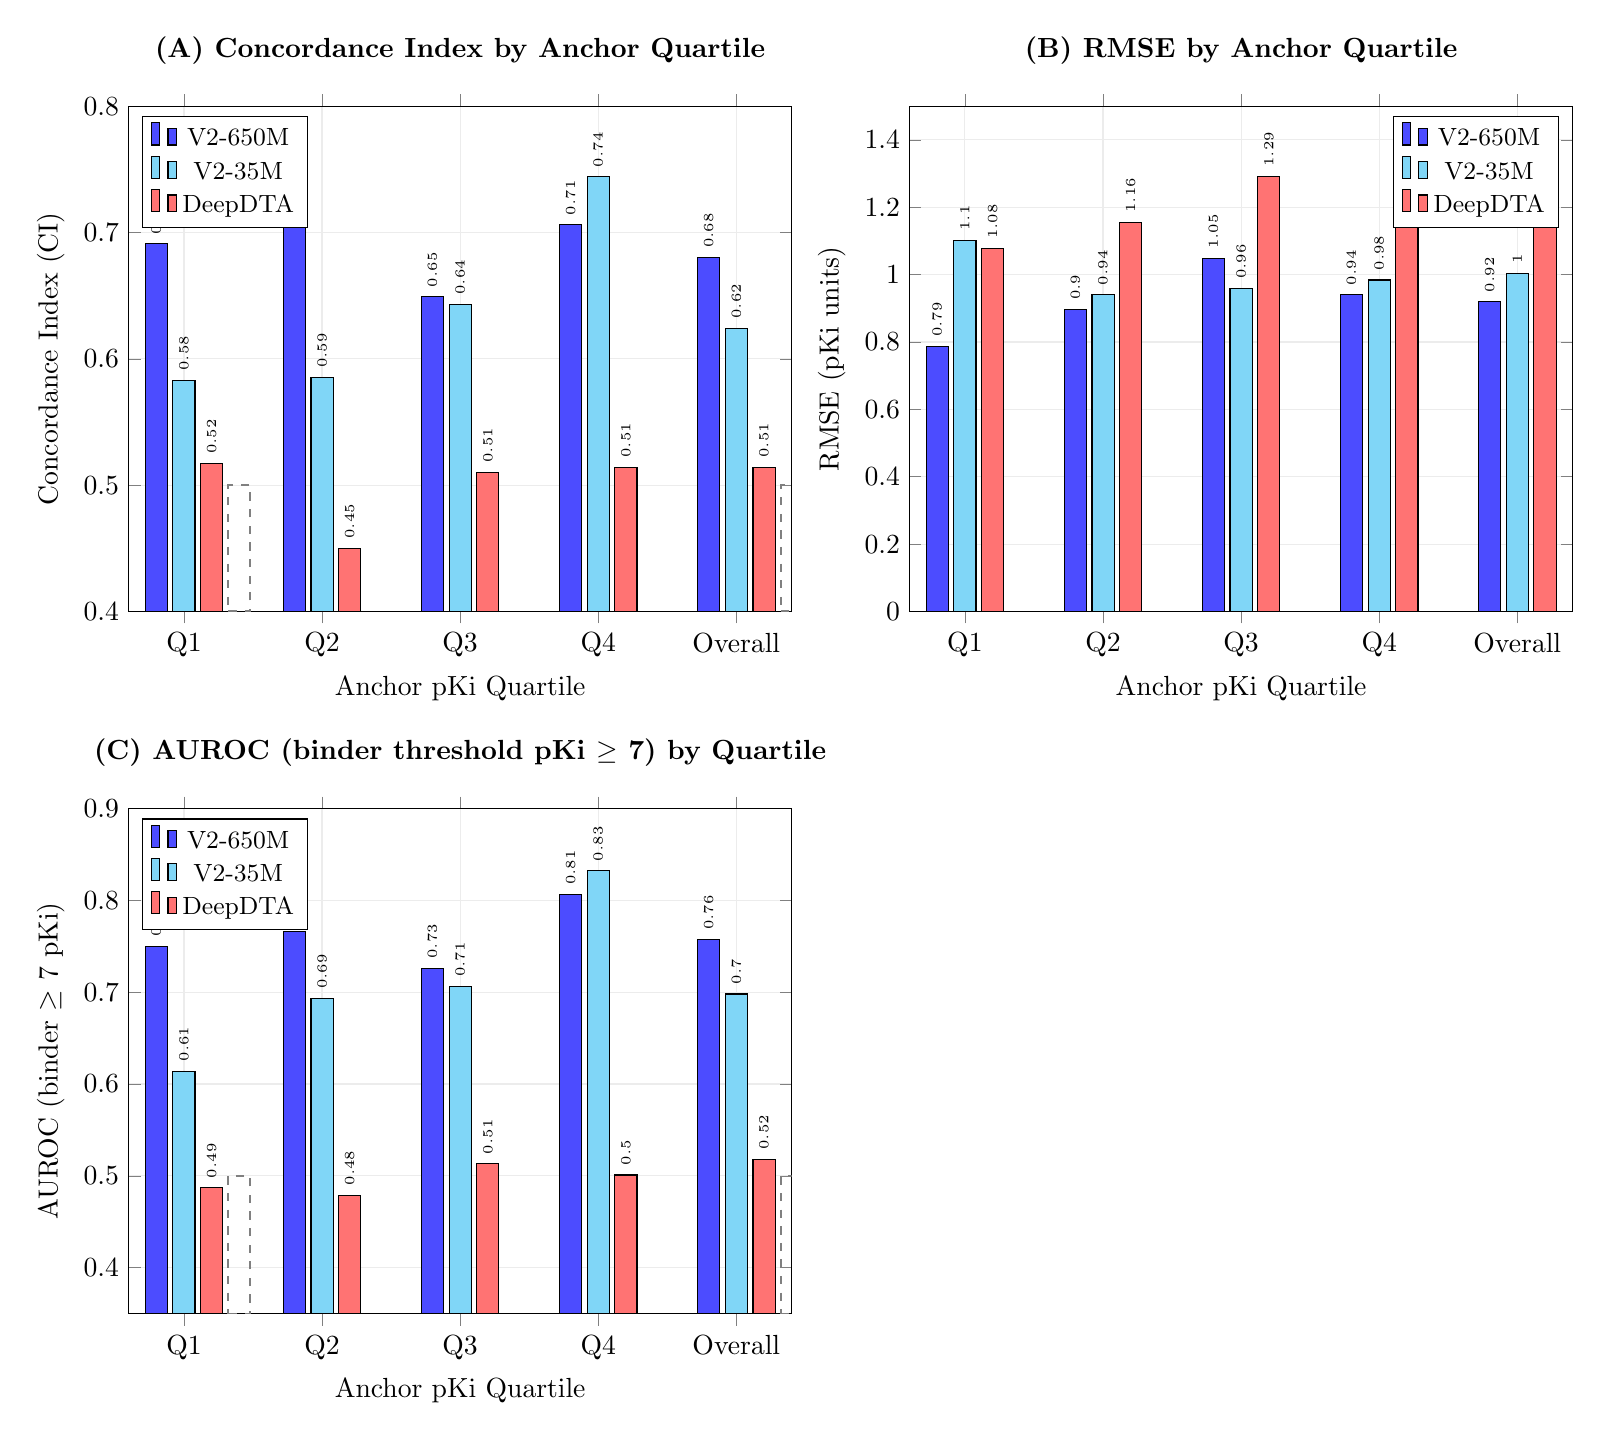
\begin{tikzpicture}

\begin{axis}[
    name=panelA, ybar, bar width=8pt, width=10cm, height=8cm,
    ylabel={Concordance Index (CI)}, xlabel={Anchor pKi Quartile},
    symbolic x coords={Q1, Q2, Q3, Q4, Overall}, xtick=data,
    ymin=0.40, ymax=0.80,
    legend style={at={(0.02,0.98)}, anchor=north west, font=\small},
    title={\textbf{(A) Concordance Index by Anchor Quartile}},
    title style={font=\normalsize, at={(0.5,1.03)}, anchor=south},
    grid=major, grid style={gray!15}, ymajorgrids=true,
    nodes near coords style={font=\tiny, rotate=90, anchor=west},
]
\addplot[fill=blue!70, nodes near coords] coordinates { (Q1, 0.691) (Q2, 0.706) (Q3, 0.649) (Q4, 0.706) (Overall, 0.680) };
\addplot[fill=cyan!50, nodes near coords] coordinates { (Q1, 0.583) (Q2, 0.585) (Q3, 0.643) (Q4, 0.744) (Overall, 0.624) };
\addplot[fill=red!55, nodes near coords] coordinates { (Q1, 0.517) (Q2, 0.450) (Q3, 0.510) (Q4, 0.514) (Overall, 0.514) };
\legend{V2-650M, V2-35M, DeepDTA}
\addplot[dashed, gray, thick, forget plot] coordinates {(Q1, 0.5) (Overall, 0.5)};
\node[font=\small, gray, anchor=north] at (axis cs:Q1, 0.40) {[7.0--8.7]};
\node[font=\small, gray, anchor=north] at (axis cs:Q2, 0.40) {[8.7--9.1]};
\node[font=\small, gray, anchor=north] at (axis cs:Q3, 0.40) {[9.1--9.5]};
\node[font=\small, gray, anchor=north] at (axis cs:Q4, 0.40) {[9.6--10.8]};
\end{axis}

\begin{axis}[
    at={(panelA.east)}, anchor=west, xshift=1.5cm,
    ybar, bar width=8pt, width=10cm, height=8cm,
    ylabel={RMSE (pKi units)}, xlabel={Anchor pKi Quartile},
    symbolic x coords={Q1, Q2, Q3, Q4, Overall}, xtick=data,
    ymin=0.0, ymax=1.5,
    legend style={at={(0.98,0.98)}, anchor=north east, font=\small},
    title={\textbf{(B) RMSE by Anchor Quartile}},
    title style={font=\normalsize, at={(0.5,1.03)}, anchor=south},
    grid=major, grid style={gray!15}, ymajorgrids=true,
    nodes near coords style={font=\tiny, rotate=90, anchor=west},
]
\addplot[fill=blue!70, nodes near coords] coordinates { (Q1, 0.786) (Q2, 0.896) (Q3, 1.047) (Q4, 0.940) (Overall, 0.919) };
\addplot[fill=cyan!50, nodes near coords] coordinates { (Q1, 1.102) (Q2, 0.940) (Q3, 0.958) (Q4, 0.984) (Overall, 1.004) };
\addplot[fill=red!55, nodes near coords] coordinates { (Q1, 1.077) (Q2, 1.155) (Q3, 1.292) (Q4, 1.271) (Overall, 1.199) };
\legend{V2-650M, V2-35M, DeepDTA}
\end{axis}

\begin{axis}[
    at={(panelA.south west)}, anchor=north west, yshift=-2.5cm,
    ybar, bar width=8pt, width=10cm, height=8cm,
    ylabel={AUROC (binder $\geq$ 7 pKi)}, xlabel={Anchor pKi Quartile},
    symbolic x coords={Q1, Q2, Q3, Q4, Overall}, xtick=data,
    ymin=0.35, ymax=0.90,
    legend style={at={(0.02,0.98)}, anchor=north west, font=\small},
    title={\textbf{(C) AUROC (binder threshold pKi $\geq$ 7) by Quartile}},
    title style={font=\normalsize, at={(0.5,1.03)}, anchor=south},
    grid=major, grid style={gray!15}, ymajorgrids=true,
    nodes near coords style={font=\tiny, rotate=90, anchor=west},
]
\addplot[fill=blue!70, nodes near coords] coordinates { (Q1, 0.750) (Q2, 0.766) (Q3, 0.726) (Q4, 0.806) (Overall, 0.757) };
\addplot[fill=cyan!50, nodes near coords] coordinates { (Q1, 0.614) (Q2, 0.693) (Q3, 0.706) (Q4, 0.832) (Overall, 0.698) };
\addplot[fill=red!55, nodes near coords] coordinates { (Q1, 0.487) (Q2, 0.479) (Q3, 0.513) (Q4, 0.501) (Overall, 0.518) };
\legend{V2-650M, V2-35M, DeepDTA}
\addplot[dashed, gray, thick, forget plot] coordinates {(Q1, 0.5) (Overall, 0.5)};
\end{axis}

\end{tikzpicture}
\end{document}
